\documentclass[tikz]{standalone}
\usepackage{pgfplots}
\pgfplotsset{compat=1.15}
\usepackage{mathrsfs}
\usetikzlibrary{arrows,calc}
\usepackage{tkz-euclide}
\pagestyle{empty}

\definecolor{AngleClr}{rgb}{0,0.39215686274509803,0}
\definecolor{ShapeClr}{rgb}{0.6,0.2,0}

\begin{document}

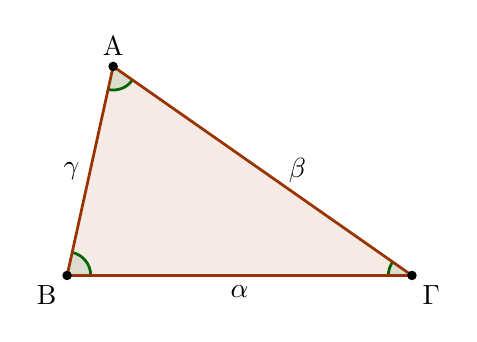
\begin{tikzpicture}[scale=.75]
\tkzSetUpLine[line width=1pt,color=black]
\tkzSetUpPoint[fill=black]

\tkzDefPoints{-3.5/0.84/A,-4.28/-2.7/B,1.56/-2.7/C}


\tkzFillPolygon[fill=ShapeClr,fill opacity=0.1](A,B,C)
\tkzFillAngles[fill=AngleClr,size=.4,fill opacity=0.1](C,B,A A,C,B B,A,C)
\tkzMarkAngles[line width=1pt,size=.4,color=AngleClr](C,B,A A,C,B B,A,C)

\tkzDrawPolygon[color=ShapeClr](A,B,C)
\tkzDrawPoints[size=3](A,B,C)
\tkzLabelPoint[above](A){$\rm A$}
\tkzLabelPoint[below left](B){$\rm B$}
\tkzLabelPoint[below right](C){$\rm \Gamma$};

\tkzLabelSegment[below](B,C){$\alpha$}
\tkzLabelSegment[right=0.2cm](A,C){$\beta$}
\tkzLabelSegment[left](A,B){$\gamma$}

\end{tikzpicture}

\end{document}
